\subsection{Limitations}
\label{sec:omp:limitations}

\todorev{Revised and finished on Sat, June 30 at 22:49 by pfac}

The main problem with this implementation is data locality.
While these issues are softened using a SOA approach, and the method is a first order one, the algorithm is still not very cache friendly in either of the core functions.

In \computeflux, each edge requires access to data from the two adjacent cells. While the access to edges is contiguous here, access to cells is not for most of the iterations. Yet, border edges do not require the second edge.

\update on the other hand requires access to all the edges in a cell, which are always more than two.
Analogously, the access to cells here is contiguous, but the access to edges is not.
Since there are more edges per cell than there are cells per edge, this function is most likely the bottleneck of the main loop.

The locality issues may be improved by changing how the mesh is built.
The generator used for this project (\texttt{gmsh}) does not optimize the mesh locality (see \cref{fig:locality}).

Alternatively, works from other authors were found to improve this issue (the most promising being \cite{hoppe99}), but the complexity behind studying a new approach to the problem and implementing it could push the project beyond the time limitations.

Similarly, a specialized library to work with meshes was found \cite{metis}.
While it could dramatically improve the mesh structure, just like using other authors' works, setting up the library and learning how to use it properly could take more time beyond the limits of the project.

\begin{figure}[!htp]
	\centering
	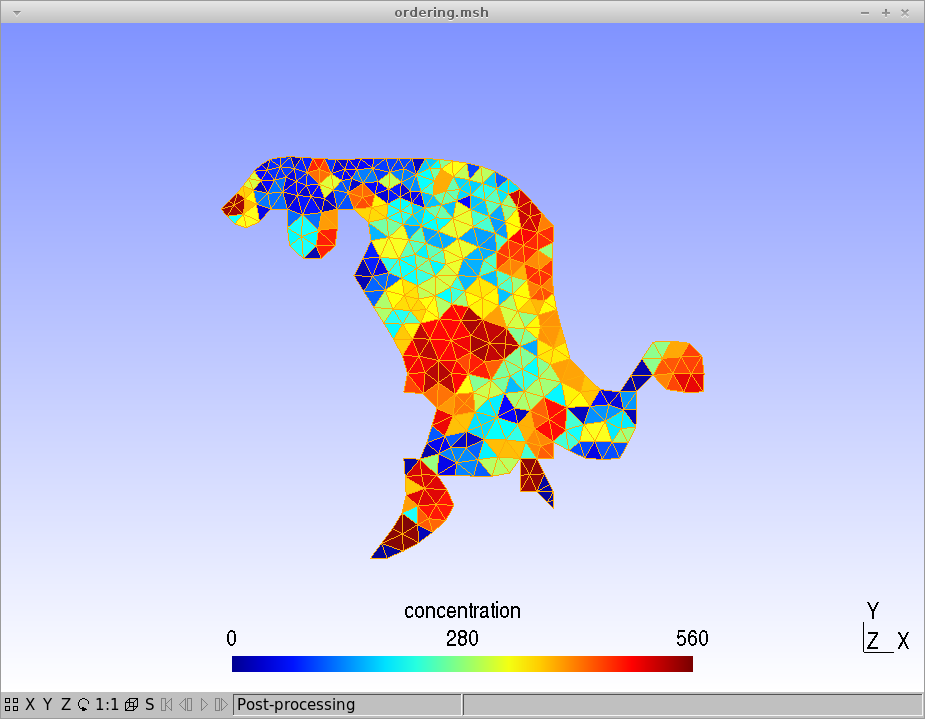
\includegraphics[width=\columnwidth]{locality_tiny.png}
	\caption{Cell locality in the mesh used as test case in this document (with increased granularity, to make it visible). The more different the colors, the more distant the cells are in the data structure.}
	\label{fig:locality}
\end{figure}
